% Foliensatz: "AFu-Kurs nach DJ4UF" von DK0TU, Amateurfunkgruppe der TU Berlin
% Lizenz: CC BY-NC-SA 3.0 de (http://creativecommons.org/licenses/by-nc-sa/3.0/de/)
% Autoren: Felix Baum <baum@campus.tu-berlin.de>

preamble.dk0tu.tex
\subtitle{Technik 15: \\
           Sender- und Empfängertechnik \\[2em]}
\date{Stand 12.1.2015}
 \begin{document}

\begin{frame}
    \titlepage
    \vfill
    \begin{center}
        \ccbyncsaeu\\
        {\tiny This work is licensed under the \em{Creative Commons Attribution-NonCommercial-ShareAlike 3.0 License}.}\\[0.5ex]
         \tiny Amateurfunkgruppe der Technische Universität Berlin (AfuTUB), DKØTU
         %\includegraphics[scale=0.5]{img/DK0TU_Logo.pdf}
    \end{center}
\end{frame}


%fixme Referenzen/Fußnoten-Systematik vereinheitlichen

\section*{Einleitung}

\begin{frame}
    \frametitle{Was ist das?}
		\begin{center}
        	\includegraphics[width=.95\textwidth]{e15/bitx.png}
        \footnote{\tiny \url{http://www.phonestack.com/farhan/bitx.html}}
	\end{center}
\end{frame}

\begin{frame}
    \frametitle{In freier Wildbahn}
    \begin{itemize}
		\item Wo findet man Sender?
		\item Wo findet man Empfänger?
    \end{itemize}
\end{frame}

\begin{frame}
    \frametitle{Funktion}
    \begin{center}
        \includegraphics[width=1\textwidth]{e15/TRX-superSimple.png}
        \footnote{\tiny \url{https://en.wikipedia.org/wiki/File:Signal_processing_system.png}}
	\end{center}
\end{frame}
  
\section*{Sender}

\begin{frame}
    \frametitle{Sender - Blockschaltbild}
    \begin{center}
        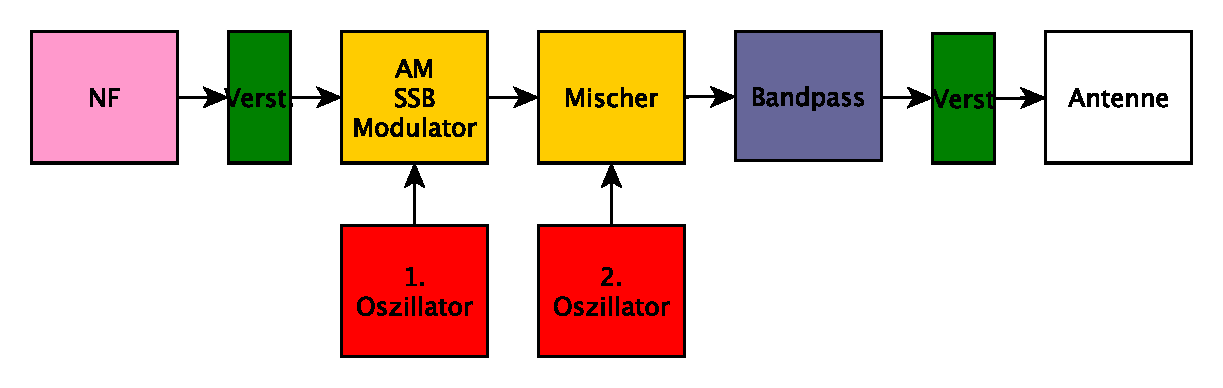
\includegraphics[width=1\textwidth]{e15/ssb-trx-bsb.pdf}
        \footnote{\tiny DB4UM}
	\end{center}
\end{frame}

\begin{frame}
    \frametitle{Sender}
    \begin{center}
        \includegraphics[width=.95\textwidth]{e15/bitx-farbe.png}
        \footnote{\tiny \url{http://www.phonestack.com/farhan/bitx.html}}
	\end{center}
\end{frame}

\section*{Oszillator}

\begin{frame}
    \frametitle{Oszillator}
    \begin{center}
    \begin{itemize}
			\item VCO
			\begin{itemize}
				\item Voltage Controlled Oszillator
				\item Auch VFO (Variable Frequency Oszillator)
				\item Spannungsabhängiger Oszillator \\ ""
   			\end{itemize}
			\item BFO
			\begin{itemize}
				\item Beat Frequency Oszillator
				\item Möglichst Frequenzstabiel auf einer Frequenz
    		\end{itemize}
    \end{itemize}
	\end{center}
\end{frame}

\begin{frame}
    \frametitle{Prüfungsfrage}

    \begin{center}
    \begin{tabular}{l||l}\hline
        TD604 &Wie verhält sich die Frequenz eines LC-Oszillators \\
         " "  & bei Temperaturanstieg, wenn die Kapazität \\
         " "  & des Schwingkreiskondensators mit dem \\
         " "  & Temperaturanstieg geringer wird? \\ \hline\hline
         A & Die Frequenz wird niedriger. \\\hline
         B & Die Frequenz bleibt stabil. \\\hline
         C & Die Frequenz wird erhöht. \\ \hline
         D & Die Schwingungen reißen ab (Aussetzer).\\\hline
    \end{tabular}
 	\end{center}
\end{frame}

\begin{frame}
    \frametitle{Prüfungsfrage}

    \begin{center}
    \begin{tabular}{l||l}\hline
        TD604 &Wie verhält sich die Frequenz eines LC-Oszillators \\
         " "  & bei Temperaturanstieg, wenn die Kapazität \\
         " "  & des Schwingkreiskondensators mit dem \\
         " "  & Temperaturanstieg geringer wird? \\ \hline\hline
         " " & Die Frequenz wird niedriger. \\\hline
         " " & Die Frequenz bleibt stabil. \\\hline
         X & Die Frequenz wird erhöht. \\ \hline
         " " & Die Schwingungen reißen ab (Aussetzer).\\\hline
    \end{tabular}
 	\end{center}
\end{frame}

\begin{frame}
    \frametitle{Oszillator}
    \begin{center}
    \begin{itemize}
			\item Warum ist es so schwierig einen Frequenzstabielen BFO zu bauen?
			\item Was für Möglichkeiten gibt es?
    \end{itemize}
	\end{center}
\end{frame}

\section*{Mischer}

\begin{frame}
    \frametitle{Mischer}
    \begin{center}
        \includegraphics[width=1\textwidth]{e15/IdealerMischer.png}
        \footnote{\tiny \url{https://commons.wikimedia.org/wiki/File:Mischer.svg}}
	\end{center}
\end{frame}

\begin{frame}
    \frametitle{Realer Diodenmischer}
    \begin{center}
        \includegraphics[width=.9\textwidth]{e15/Realer-Diodenmischer.png}
        \footnote{\tiny \url{https://commons.wikimedia.org/wiki/File:Diode_DBM.png}}
	\end{center}
\end{frame}

\begin{frame}
    \frametitle{Mischer Rechenübung}
    \begin{center}
    \begin{itemize}
			\item Oszillator 1: $10 MHz$
			\item Oszillator 2: $4.1 MHz$ \\ " "
			\item Welche Ausgangsfrequenzen?
    \end{itemize}
	\end{center}
\end{frame}

\begin{frame}
    \frametitle{Prüfungsfrage}

    \begin{center}
    \begin{tabular}{l||l}\hline
        TF107 &Einem Mischer werden die Frequenzen 28 MHz\\
         " "  &und 38,7 MHz zugeführt. Welche Frequenzen\\
         " "  &werden beim Mischvorgang erzeugt?\\ \hline\hline
         A & 10,7 MHz und 56 MHz \\\hline
         B & 10,7 MHz \\\hline
         C & 56 MHz und 66,7 MHz \\ \hline
         D & 10,7 MHz und 66,7 MHz\\\hline
    \end{tabular}
 	\end{center}
\end{frame}

\begin{frame}
    \frametitle{Prüfungsfrage}
    \begin{center}
    \begin{tabular}{l||l}\hline
        TF107 &Einem Mischer werden die Frequenzen 28 MHz\\
         " "  &und 38,7 MHz zugeführt. Welche Frequenzen\\
         " "  &werden beim Mischvorgang erzeugt? \\ \hline\hline
         " " & 10,7 MHz und 56 MHz \\\hline
         " " & 10,7 MHz \\\hline
         " " & 56 MHz und 66,7 MHz \\ \hline
         X & 10,7 MHz und 66,7 MHz\\\hline
    \end{tabular}
    Hinweis: Die ungewollte Frequenz heißt auch Spiegelfrequenz.
 	\end{center}
\end{frame}

\section*{Transverter}

\begin{frame}
    \frametitle{Transverter - Blockschaltbild}
    \begin{center}
        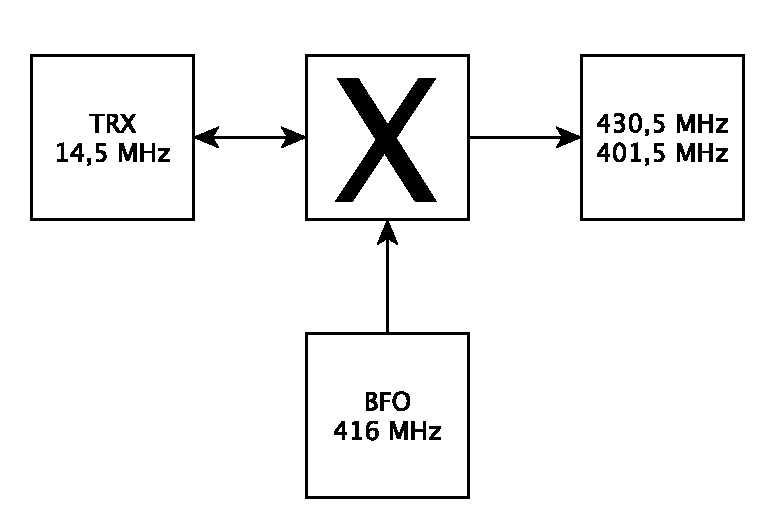
\includegraphics[width=1\textwidth]{e15/transverter.pdf}
	\end{center}
\end{frame}

\section*{Empfänger}

\begin{frame}
    \frametitle{Direktüberlagerungsempfänger - Blockschaltbild}
    \begin{center}
        \includegraphics[width=.99\textwidth]{e15/Ueberlagerungsempfanger_blockschaltbild.png}
        \footnote{\tiny \url{https://commons.wikimedia.org/wiki/File:Ueberlagerungsempfänger_blockschaltbild.svg}}
	\end{center}
\end{frame}

\begin{frame}
    \frametitle{Spiegelfrequenz}
    \begin{center}
        \includegraphics[width=.99\textwidth]{e15/Uberlagerungsempfanger_Spiegelfrequenz.png}
        \footnote{\tiny \url{https://commons.wikimedia.org/wiki/File:C3CberlagerungsempfC3A4nger_Spiegelfrequenz.png}}
	\end{center}
\end{frame}

\section*{Sonstiges}
\begin{frame}
    \frametitle{SNR}
    \begin{itemize}
		\item Das Signal-Rausch-Verhältnis dient als Bewertungszahl zur Beurteilung der Qualität eines (analogen) Kommunikationspfades.
		\item Um Sprache verstehen zu können braucht es ein SNR von ca 6dB
    \end{itemize}
\end{frame}

\begin{frame}
    \frametitle{Trennschärfe}
    \begin{itemize}
		\item Beurteilt wie gut der Empfänger ein Signal von starken benachbarten Signalen trennen kann.
		\item Je steiler der Bandpass, desto besser die Trennschärfe
    \end{itemize}
\end{frame}

\begin{frame}
    \frametitle{Großsignalfestigkeit}
    \begin{itemize}
		\item Beurteilt wie gut der Empfänger mit ganz starken Signalen zurechtkommt
		\item Bekannt ist z.B. dann ein zugestopft des Empfängers bei zu starken Signalen (Erkennbar durch brummen)
    \end{itemize}
\end{frame}

\section*{Transciver}

\begin{frame}
    \frametitle{BITX}
        \includegraphics[width=1.02\textwidth]{e15/bitx-farbe.png}
        \footnote{\tiny \url{http://www.phonestack.com/farhan/bitx.html}}
\end{frame}

\begin{frame}
    \frametitle{Elecraft - K3}
        \begin{center}
        \includegraphics[width=1.22\textwidth]{e15/K3_Front.jpg}
        \footnote{\tiny \url{http://www.elecraft.com/K3/K3.htm}}
	\end{center}
\end{frame}

\begin{frame}
    \frametitle{Drake TR-7}
        \begin{center}
        \includegraphics[width=1.22\textwidth]{e15/drake.jpg}
        \footnote{\tiny Bild von DB4UM bei DK0TU}
	\end{center}
\end{frame}

\section*{Referenzen}

\begin{frame}
    \frametitle{Referenzen/Links}
    
    \footnotesize
    \begin{itemize}
        \item Moltrecht E 15: \\
              \url{http://www.darc.de/referate/ajw/ausbildung/darc-online-lehrgang/technik-klasse-e/technik-e15/}
        \item Überlagerungsempfänger (Wikipedia): \\
              \url{https://de.wikipedia.org/wiki/Ueberlagerungsempfaenger}
    \end{itemize}

\end{frame}

% Hier könnte noch eine Kontaktfolie stehen

\end{document}

